\chapter{Metodología} \label{ch:metodologia}

\section{Herramientas utilizadas}

El diseño del procesador base utilizado se encuentra en el repositorio riscv-vhdl \cite{base_riscv_cpu_git}. Para definir la extensión del procesador RISC-V se ha utilizado el lenguaje de especificación hardware VHDL. Para simular el comportamiento del procesador se ha utilizado el simulador GHDL \cite{ghdl} junto con el visor de ondas GTKWave \cite{gtkwave}. Los programas que se han ejecutado en los procesadores simulados se han desarrollado en C y para compilarlos se ha utilizado el conjunto de herramientas GNU RISC-V Compiler Toolchain \cite{gcc_riscv}.

Para entrenar BNNs se ha utilizado la biblioteca de Python TensorFlow Probability \cite{tfprob} junto al repositorio BNN\_for\_hyperspectral\_datasets\_analysis \cite{bnn_hyper_git}. El proceso de compilación y pruebas se han automatizado todo lo posible mediante la herramienta Make y \textit{scripts} en Bash y Python. Para manejar ficheros ELF desde Python se ha utilizado la biblioteca pyelftools \cite{pyelftools}. Para crear gráficas se ha utilizado la biblioteca de Python Matplotlib \cite{matplotlib}. Se han utilizado los test estadísticos de la biblioteca de Python SciPy \cite{scipy}.

Se ha utilizado la plataforma de desarrollo Xilinx ZCU104 FPGA \cite{fpga_board} junto a Vivado Design Suite \cite{vivado} para implementar los diseños hardware sobre una FPGA y analizar sus costes.

Para redactar este documento se ha utilizado el editor de \LaTeX\ en línea Overleaf \cite{overleaf} y para crear los diagramas se utilizado el editor en línea draw.io \cite{drawio} junto al editor de gráficos vectoriales Inkscape \cite{inkscape}.

Como programa de control de versiones se ha utilizado Git \cite{git} junto con GitHub \cite{github} como repositorio en línea.

\section{Modelos utilizados}

Durante el proceso de verificación se han utilizado tres arquitecturas de modelos diferentes. Estos modelos se han elegido por que han sido utilizados por otros trabajos recientes o por que son arquitecturas estándar muy conocidas. La Tabla \ref{tab:hyper_models} muestra la arquitectura de los modelos para clasificación de píxeles hiperespectrales \cite{bnn_hyper_uncertainty}. Los conjuntos de datos utilizados para este modelo son diferentes imágenes hiperespectrales obtenidas mediante satélite denominadas BO, IP, KSC, PU y SV.

%%%%

\begin{table}[h]
	\centering
	\caption{Arquitectura de los modelos para clasificación de píxeles hiperespectrales.}
	\label{tab:hyper_models}
	\begin{tabular}{lll}
	\hline
     	\textbf{Tipo de capa} & \textbf{Entrada} & \textbf{Salida}\\ \hline
     	Dense ReLU& Número de bandas espectrales & 32\\
     	Dense ReLU& 32 & 16\\
     	Dense SoftMax& 16 & Número de clases de píxeles\\ \hline
	\end{tabular}
\end{table}

La Tabla \ref{tab:cnn_models} muestra una arquitectura LeNet-5 bayesiana. LeNet-5 es una arquitectura de red neuronal convolucional (\textit{\textbf{C}onvolutional \textbf{N}eural \textbf{N}etwork}) simple \cite{lenet}. Se ha entrenado un modelo con la misma arquitectura para reconocer el conjunto de datos MNIST \cite{MNIST_dataset} y CIFAR-10 \cite{CIFAR_dataset} pero utilizando capas bayesianas.

\begin{table}[h]
	\centering
	\caption{Arquitectura LeNet-5 bayesiana.}
	\label{tab:cnn_models}
	\begin{tabular}{llll}
    	\hline
     	\textbf{Tipo de capa} &  \textbf{Entrada} &  \textbf{Salida} & \textbf{Tamaño del filtro} \\ \hline
     	Conv2D Valid ReLU& 28$\times$28 & 24$\times$24$\times$6 & 5$\times$5 \\
     	MaxPool2D & 24$\times$24$\times$6 & 12$\times$12$\times$6 & 2$\times$2 \\
     	Conv2D Valid  ReLU& 12$\times$12$\times$6 & 8$\times$8$\times$16 & 5$\times$5 \\
     	MaxPool2D & 8$\times$8$\times$16 & 4$\times$4$\times$16 & 2$\times$2 \\
     	Conv2D Valid  ReLU& 4$\times$4$\times$16 & 1$\times$1$\times$120 & 4$\times$4 \\
     	Dense ReLU& 120 & 84 & \\
     	Dense SoftMax& 84 & 10 & \\ \hline
	\end{tabular}
\end{table}

La Tabla \ref{tab:b2n2_model} muestra la arquitectura B2N2, propuesta por Awano \emph{et al.} junto a su acelerador para BNN \cite{bnn_clt_approx}. También se ha entrenado para reconocer los conjuntos de datos MNIST y CIFAR-10.

\begin{table}[h]
	\centering
	\caption{Arquitectura B2N2.}
	\label{tab:b2n2_model}
	\begin{tabular}{llll}
	\hline
	\textbf{Tipo de capa} & \textbf{Entrada} & \textbf{Salida} & \textbf{Tamaño del filtro}\\ \hline
	Conv2D Same ReLU& 32$\times$32 & 32$\times$32$\times$32 & 3$\times$3 \\
	Conv2D Same  ReLU& 32$\times$32$\times$32 & 32$\times$32$\times$32 & 3$\times$3 \\
	MaxPool2D & 32$\times$32$\times$32 & 16$\times$16$\times$32 & 2$\times$2 \\
	Conv2D Same  ReLU& 16$\times$16$\times$32 & 16$\times$16$\times$64 & 3$\times$3 \\
	Conv2D Same  ReLU& 16$\times$16$\times$64 & 16$\times$16$\times$64 & 3$\times$3 \\
	MaxPool2D & 16$\times$16$\times$64 & 8$\times$8$\times$64 & 2$\times$2 \\
	Conv2D Same  ReLU& 8$\times$8$\times$64 & 8$\times$8$\times$128 & 3$\times$3 \\
	Conv2D Same  ReLU& 8$\times$8$\times$128 & 8$\times$8$\times$128 & 3$\times$3 \\
	MaxPool2D & 8$\times$8$\times$128 & 4$\times$4$\times$128 & 2$\times$2 \\
	Dense SoftMax& 2028 & 10 & \\ \hline
	\end{tabular}
\end{table}

\section{Configuración experimental}

La Figura \ref{fig:experiment_pipeline} muestra el proceso y componentes para ejecutar inferencia de BNN de manera eficiente en un procesador RISC-V con soporte único para precisión entera que se han utilizado para obtener los resultados de este trabajo.

\begin{figure}[h]
	\centering
	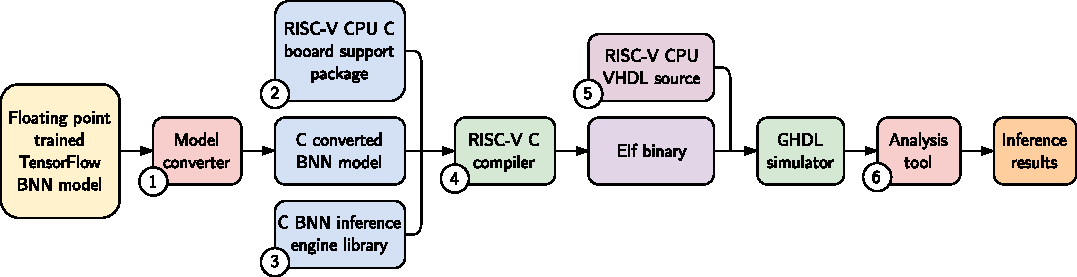
\includegraphics[width=\textwidth]{root/Imagenes/metodologia/experiment_pipeline.pdf}
	\caption{Diagrama de componentes necesarios para ejecutar la inferencia de BNN en un procesador RISC-V simulado. Los componentes marcados con un número son contribuciones de este trabajo.}
	\label{fig:experiment_pipeline}
\end{figure}

\subsection{Conversor de modelos}

Se ha desarrollado una herramienta en Python, marcada en la Figura \ref{fig:experiment_pipeline} como componente 1, que convierte modelos BNN TensorFlow ya entrenados en precisión de punto flotante a ficheros de código C con precisión en coma fija que puedan ejecutarse junto al motor de inferencia explicado en el Capítulo \ref{ch:motor_inferencia}. La Figura \ref{fig:model_converter} muestra un diagrama de las diferentes operaciones que realiza esta herramienta.

\begin{figure}[h]
	\centering
	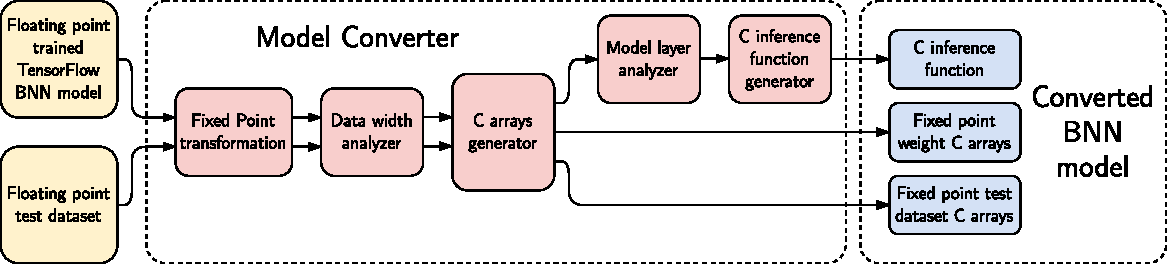
\includegraphics[width=\textwidth]{root/Imagenes/metodologia/model_converter.pdf}
	\caption{Diagrama de componentes internos del conversor de modelos.}
	\label{fig:model_converter}
\end{figure}

Primero aplica transformaciones a los pesos requeridas por las optimizaciones detalladas en el Capítulo \ref{ch:optimizaciones} utilizando coma flotante para tener la máxima precisión posible, tras ello codifica los valores en coma fija utilizando una escala constante previamente definida. A continuación analiza el número de bits necesarios para almacenar los datos y selecciona los datos nativos de C con los bits necesarios, seguidamente almacena todos los pesos en vectores de C. Finalmente analiza la función de inferencia del modelo y crea una versión en C utilizando las funciones proporcionadas por el motor de inferencia.

\subsubsection{Precisión en coma fija}

Implementar aritmética de coma flotante en hardware es caro, por lo que es común que procesadores de bajas prestaciones no dispongan de dicho hardware. GCC permite emular las operaciones de coma flotante mediante software, comúnmente conocido como \textit{soft-float}. Esta emulación tiene un gran impacto en el rendimiento por lo que no se ha utilizado.

Para mejorar el rendimiento, se ha adoptado el formato de coma fija para la representación de números decimales. Este formato permite realizar operaciones con números decimales utilizando hardware de precisión entera, lo que tiene un impacto mínimo en el rendimiento. Esta codificación consiste en multiplicar los números con una escala potencia de 2. A mayor sea la escala mayor precisión se obtiene. La principal limitación de esta codificación es el tamaño de palabra de la arquitectura ya que pueden ocurrir desbordamientos al operar con números multiplicados por una escala grande. Por lo que en general se obtiene menor precisión que con la codificación en punto flotante. La Figura \ref{fig:fixed_point} muestra un ejemplo de este tipo de codificación.

\begin{figure}[h]
	\centering
	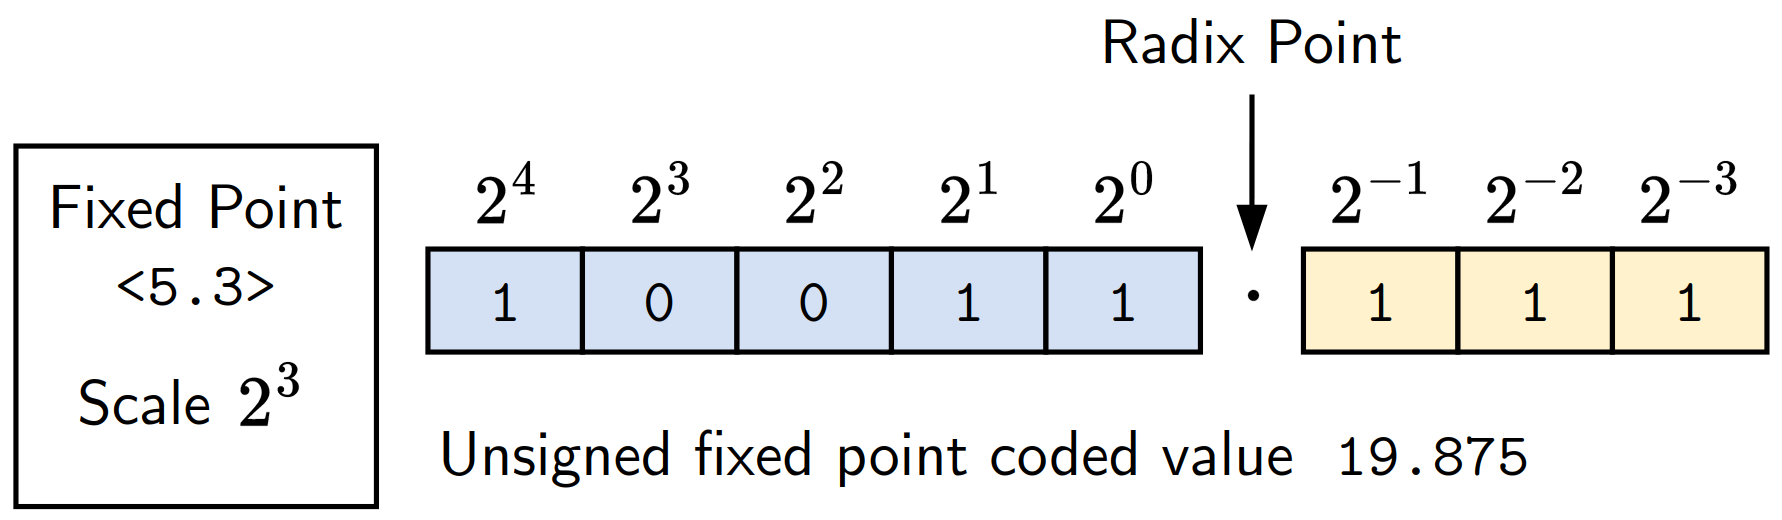
\includegraphics[width=0.7\textwidth]{root/Imagenes/metodologia/fixed_point.png}
	\caption{Ejemplo de codificación en coma fija sin signo \texttt{<5.3>} del valor 19.875.}
	\label{fig:fixed_point}
\end{figure}

\subsection{Actualización del Board Support Package}

El \textit{\textbf{B}oard \textbf{S}upport \textbf{P}ackage} (BSP) de una plataforma es una capa de software intermedia entre la aplicación y el hardware que contiene código específico para crear un entorno de ejecución estable en dicha plataforma. Además puede proveer de los ficheros de configuración y un sistema de compilación. En la Figura \ref{fig:experiment_pipeline} aparece componente 2. En la Figura \ref{fig:bsp} se muestra un diagrama con más detalle sobre este componente.

\begin{figure}[h]
	\centering
	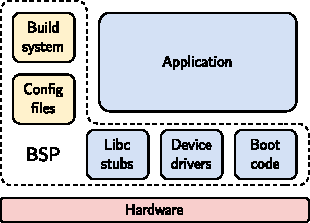
\includegraphics[width=0.6\textwidth]{root/Imagenes/metodologia/bsp.pdf}
	\caption{Diagrama de componentes que forman un BSP y cómo se sitúa entre la aplicación y el hardware.}
	\label{fig:bsp}
\end{figure}

Con el objetivo de mejorar la experiencia de desarrollo del motor de inferencia se actualizó el BSP del procesador para dar soporte a la biblioteca estándar C (libc) y algunas funcionalidades de C++. De esta forma se pueden utilizar funciones útiles de libc cómo \texttt{printf}, o \texttt{memset} entre otras. Para ello se actualizaron las herramientas y ficheros de compilación, se añadieron funciones \textit{stub} para las llamadas al sistema no implementadas y se implementaron versiones modificadas de \texttt{\_write} y \texttt{\_exit}.

\subsection{Verificación}

Para validar el correcto funcionamiento del motor de inferencia y estudiar el impacto en el rendimiento de las optimizaciones posteriores se ha desarrollado una herramienta que compara las predicciones del conjunto de datos de prueba obtenidas con el motor de inferencia y TensorFlow. Las predicciones obtenidas con TensorFlow se han tomado como punto de referencia correcto. Este componente aparece en la Figura \ref{fig:experiment_pipeline} como componente 6.

Para comparar los conjuntos de predicciones se han utilizado las métricas de incertidumbre y la precisión. La precisión se puede calcular como el ratio de predicciones acertadas sobre el número total de predicciones. Analizar las métricas de incertidumbre y las propiedades estadísticas de los modelos es complejo. Para hacerlo se han utilizado 4 tipos de gráficas que las representan, estas se explicarán más adelante en la Sección \ref{sec:uncertainty_example} mediante ejemplos.
